\section{Introduction} \label{sec:intro}
% What leads to distribution of heavy elements in a galaxy
Elements heavier than hydrogen are produced through nuclear fusion. After Big Bang Nucleosynthesis, this only occurs in compact objects. The distribution of elemental abundances in the gas-phase of a galaxy is determined by a complicated combination of physical processes - stellar evolution and supernovae, gas accretion, galaxy mergers, gas outflows from stellar and AGN feedback, metal mixing and diffusion, etc.

% How present-day stellar surface abundances are linked to history of gas-phase abundances
By necessity, stars inherit the constituitive properties of the gas cloud from which they formed. Moreover, the surface abundance of stars do not change over time.\footnote{For the most part.} We therefore have the unique opportunity to examine the historical record of the gas-phase abundance of a galaxy by way of the distribution of the surface abundances of stars. Because the processes which give rise to this distribution are complex, there is almost certainly some structure in this distribution for every galaxy. However, it has only been definitively measured in the Milky Way.

% Why alpha-elements are important
The distribution of elemental abundances is a high dimensional space (\red{e.g. up to 8 billion elements by XYZ}). However, this space is highly degenerate, and so the effective number of dimensions is much smaller - even possibly compressed to just \FeH and age \citep{2019ApJ...883..177N}.

Two elements in particular have received particular interest - iron and $\alpha$-elements (elements produced through the $\alpha$-process, often tracked with just Mg). Type Ia and Type II supernovae are the main contributors of elemental enrichment. Iron is broadly produced in both types, and so its abundance is a proxy for the total metallicity of a star. $\alpha$-elements, on the other hand, are mainly produced in Type II supernovae. The ratio of $\alpha$-elements to iron is then a measure of the relative contributions of Type Ia and II to the enrichment of a parcel of gas. It has therefore become common to compress the high-dimensional abundance space to the two dimensional \FeH-\alphaFe plane.

% Observed chemical bimodality in the Milky Way
It is now well-established that, in the Milky Way, a bimodality exists in the \alphaFe{}-\FeH{} plane \citep{1996ASPC...92..307G,1998A&A...338..161F,2004AN....325....3F,2006MNRAS.367.1329R,2011A&A...535L..11A,2012A&A...545A..32A,2014A&A...562A..71B,2014ApJ...796...38N,2020MNRAS.493.2952H}. This bimodality is typically separated into the high-$\alpha$ and low-$\alpha$ sequences. The high-$\alpha$ sequence is more centrally compact and vertically extended than the low-$\alpha$ sequence. 

% Different explanations of bimodality
Naturally, many different processes that could lead to structure in the abundance plane have been discussed in the literature. They can be separated into two broad classes: (1) structure arising from internal processes, and (2) structure arising from external processes. We will summarize these classes of explanations in turn.

An early explanation of the bimodality is the two-phase gas infall model \citep{1997ApJ...477..765C,2009IAUS..254..191C,2017MNRAS.472.3637G,2019A&A...623A..60S}. In this model, the thick disk first forms rapidly from an initial infall of gas. Because the typical SFR is high, these stars are $\alpha$-enhanced. In some variants, star formation halts completely before a second supply of pristine gas falls into the Galaxy. This dilutes the gas supply from which the thin disk forms more gradually. The thin disk is then more $\alpha$-poor because its associated SFR is lower.

Another mechanism to generate structure in the abundance plane was pointed out by \citet{2009MNRAS.396..203S}, further developed by \citet{2021MNRAS.507.5882S,2023MNRAS.523.3791C}, and explored by \citet{2011ApJ...737....8L,2021MNRAS.508.4484J}. This model claims that, since stars are thought to migrate from their birth radius, there will be stars throughout the entire disk that formed in the inner disk. These $\alpha$-enhanced stars will then form the high-$\alpha$ sequence. This model and its variants also match some chemodynamic properties of the disk. One salient feature of these models is that the bimodality can result from a smooth star formation history.

Yet another explanation invoking an internal process is that the formation of clumps at high redshift are responsible for both the chemistry and dynamics of the high-$\alpha$ sequence \citep{2019MNRAS.484.3476C,2020MNRAS.492.4716B,2021MNRAS.502..260B,2023ApJ...953..128G}. Instabilities are thought to form clumps in gas-rich disks, and such clumps are seen at intermediate redshifts \citep[$z\sim2$;][]{2005ApJ...627..632E,2007ApJ...658..763E}. These clumps then self-enrich, forming $\alpha$-enhanced stars. The high-$\alpha$ sequence stops forming once the gas fraction is low enough for the instabilities to no longer arise. This model predicts that the high-$\alpha$ and low-$\alpha$ sequences form simultaneously.

Next, we turn to models which argue the bimodality results from some external influence. Early arguments were made that both the $\alpha$-enhancement of the disk and the thickening of the disk can result from gas-rich mergers \citep{2004ApJ...612..894B,2005ApJ...630..298B,2007ApJ...658...60B,2010MNRAS.402.1489R}.\footnote{See also \citet{2009MNRAS.400.1347C} for an argument invoking semi-analytic models.} These mergers lead to an enhanced SFR which leads to the $\alpha$-enhancement of the thick disk.

In cosmological simulations, which naturally include early gas-rich mergers, the situation is not as clear. Early work by \citet{2012MNRAS.426..690B} found a general separation between the thin and thick disk, though other authors found a smooth evolution \citep{2013A&A...558A...9M}. \citet{2018MNRAS.474.3629G} found what they referred to as a chemical dichotomy, and argued that it can come from either gas-rich mergers as described before or a ``compaction'' of the disk (we will return to this point later). Other authors highlight the metal content of the infalling gas, stating that the pristine gas associated with satellites can suddenly dilute or reset the disk's metallicity \citep{2020MNRAS.491.5435B,2024MNRAS.528L.122C}

The inability of a particular conceptual framework to match every minute detail of the Galaxy does not invalidate its usefulness. It is, in our view, simplistic to claim any one factor to be the cause of structure in the abundance plane -- especially given the context that much deeper, unobserved structure almost certainly exists. The goal of this work is to argue for a closer examination of a process that has been 

In this work, we revisit the idea first touched upon by \citet{1997ApJ...477..765C} that a quiescent period may have contributed to the separation of the $\alpha$-sequences. We use fully self-consistent simulations of a galaxy merger which vaguely resembles the merger between the Milky Way and GSE. Under minor changes to the orbital parameters, we show that some mergers result in bimodal abundance planes while some result in unimodal planes (i.e., abundance plane bimodalities are not generically caused by gas-rich mergers). 

We are not confident that stellar dynamics is properly modeled in our simulations, and so we leave this aspect of the system to future work.

% GSE merger explanation

% In this work, ...


Elemental enrichment is accounted for in modern galaxy formation models, though the validity of the yield tables is suspect. It is not known if the yields (i.e., the amount of metals produced by the SN) used in such models are accurate. This issue is further compounded by the fact that the mixing of metals is unresolved and is sensitive to numerical choices (e.g., Eulerian codes being generally more diffusive than Lagrangian). To make matters even worse, the inflows and outflows of gas from galaxies is sensitive to the choices of the feedback model, which has a strong impact on a galaxy's elemental history.




The last\footnote{i.e., not ongoing} significant merger was between the
proto-Milky Way disk and the {\em Gaia}-Sausage-Enceladus (GSE)
(\textcolor{red}{spell check}) satellite galaxy. The stellar debris from this
merger constitutes $\sim50\%$ \textcolor{red}{check} of the inner ($r<?\,\kpc$)
stellar halo. It may have also led to a tilted, triaxial dark matter halo
(\textcolor{red}{cite}).

The GSE merger is often invoked (\textcolor{red}{cite}) to explain the observed
bimodality in the \textcolor{red}{alpha iron} abundance plane
(\textcolor{red}{cite}). Because GSE-mass galaxies are expected to have a lower
star formation efficiency than proto-Milky Way-mass galaxies
(\textcolor{red}{cite}), the gas from GSE should be relatively metal poor. The
gas from GSE thus dilutes the gas in the proto-Milky Way, ``resetting'' the
chemical abundance of the Milky Way.

However, it has also been claimed that the \textcolor{red}{alpha iron}
bimodality can be explained through secular processes. \textcolor{red}{Sentence
explaining the basic concept.} The argument is not that the GSE merger did not
happen, but rather that it is not {\it necessary} and might not even be {\it
sufficient} to explain the bimodality. Ongoing work to detect the bimodality in
external galaxies may shed further light on the topic (\textcolor{red}{cite}).

Investigating GSE-like mergers in cosmological simulations is a rich and active
area of research. Many mergers believed to be similar to the GSE merger have
been identified in the literature (\textcolor{red}{cite}). \textcolor{red}{Blah
blah argue blah blah. And also blah blah argues blah blah.}

While much has been learned from GSE-like mergers in cosmological simulations,
they are not conducive to controlled experiments. It is possible to change the
mass of satellites through genetic modification (\textcolor{red}{Pontzen}), and
the GSE analog can be removed entirely (\textcolor{red}{Cooke cite}). However,
to our knowledge, no method has been applied to change the orbital parameters of
such a merger. It is also somehwat unclear if the circumgalactic media of
proto-Milky Way mass galaxies at $z\sim2$ are properly simulated.

In this work, we present hydrodynamic simulations of a controlled merger between
a GSE analog and the $z\sim2$ proto-Milky Way. 

\begin{figure*}
  \centering
  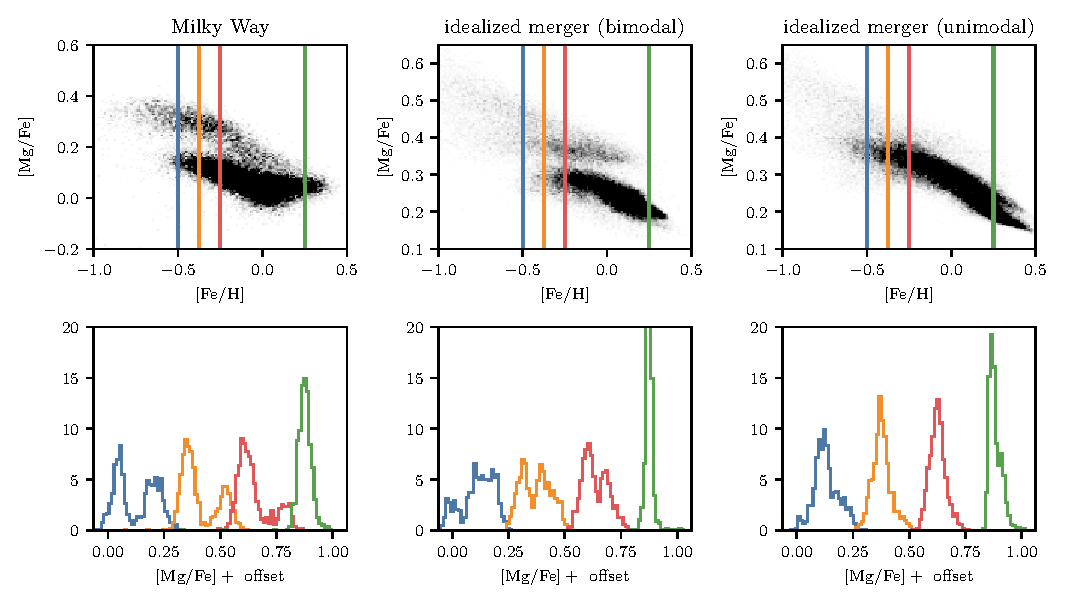
\includegraphics[width=\textwidth]{figure1.pdf}
  \caption{\textbf{The abundance bimodality seen in the Milky Way can be reproduced in some idealized merger simulations.} In the upper panels, we show the distribution of stars in the \MgFe-\FeH plane. The left panel shows the observed distribution in the Milky Way from ASPCAP \red{cite}, while the right two panels show two idealized merger simulations. The idealized merger simulations are nearly identical, except that the bimodal simulation has a starting radius of $129\,\kpc$, while the unimodal simulation has a starting radius of $142\,\kpc$. We emphasize that the labels ``unimodal'' and ``bimodal'' are of the \textit{outcome} of the simulation, and do not reflect a particular choice in the setup. The bottom panels show the distribution of \MgFe at fixed \FeH. The colors indicate the fixed \FeH values, which are $-0.5$, $-0.375$, $-0.25$, and $0.25$. The Milky Way (left panels) exhibits a strong bimodal distribution of \MgFe at various \FeH. The idealized merger simulation marked as bimodal (center panels) also exhibits a bimodal distribution of \MgFe, though the structure is not as strongly defined. The idealized merger simulation marked as unimodal exhibits only weak structure, if any at all.}
  \label{fig:fig1}
\end{figure*}